\chapter{Конструкторская часть}

В данном разделе представлена диаграмма разрабатываемой базы данных, выполнено описание ее сущностей, определены ограничения целостности, а также описаны проектируемая функция и ролевые модели.

\section{Описание сущностей и ограничений целостности}

В реализуемой базе данных выделены следующие таблицы:

\begin{itemize}[label=---]
    \item AppUser --- таблица пользователей;
    \item TrackInfo --- таблица отслеживаний маршрутов автомобилей;
    \item Car --- таблица автомобилей;
    \item CarOwner --- таблица владельцев;
    \item STS --- таблица СТС;
    \item PTS --- таблица ПТС;
    \item OwnerHistory --- таблица истории владения транспортными средствами;
    \item OwnerHistoryOwner --- таблица-связь владельцев и историй владения;
    \item Camera --- таблица дорожных камер;
    \item CarSnapshot --- таблица снимков автомобилей.
\end{itemize}

На рисунке~\ref{fig:tables} представлена диаграмма базы данных.

\begin{figure}[H]
    \centering
    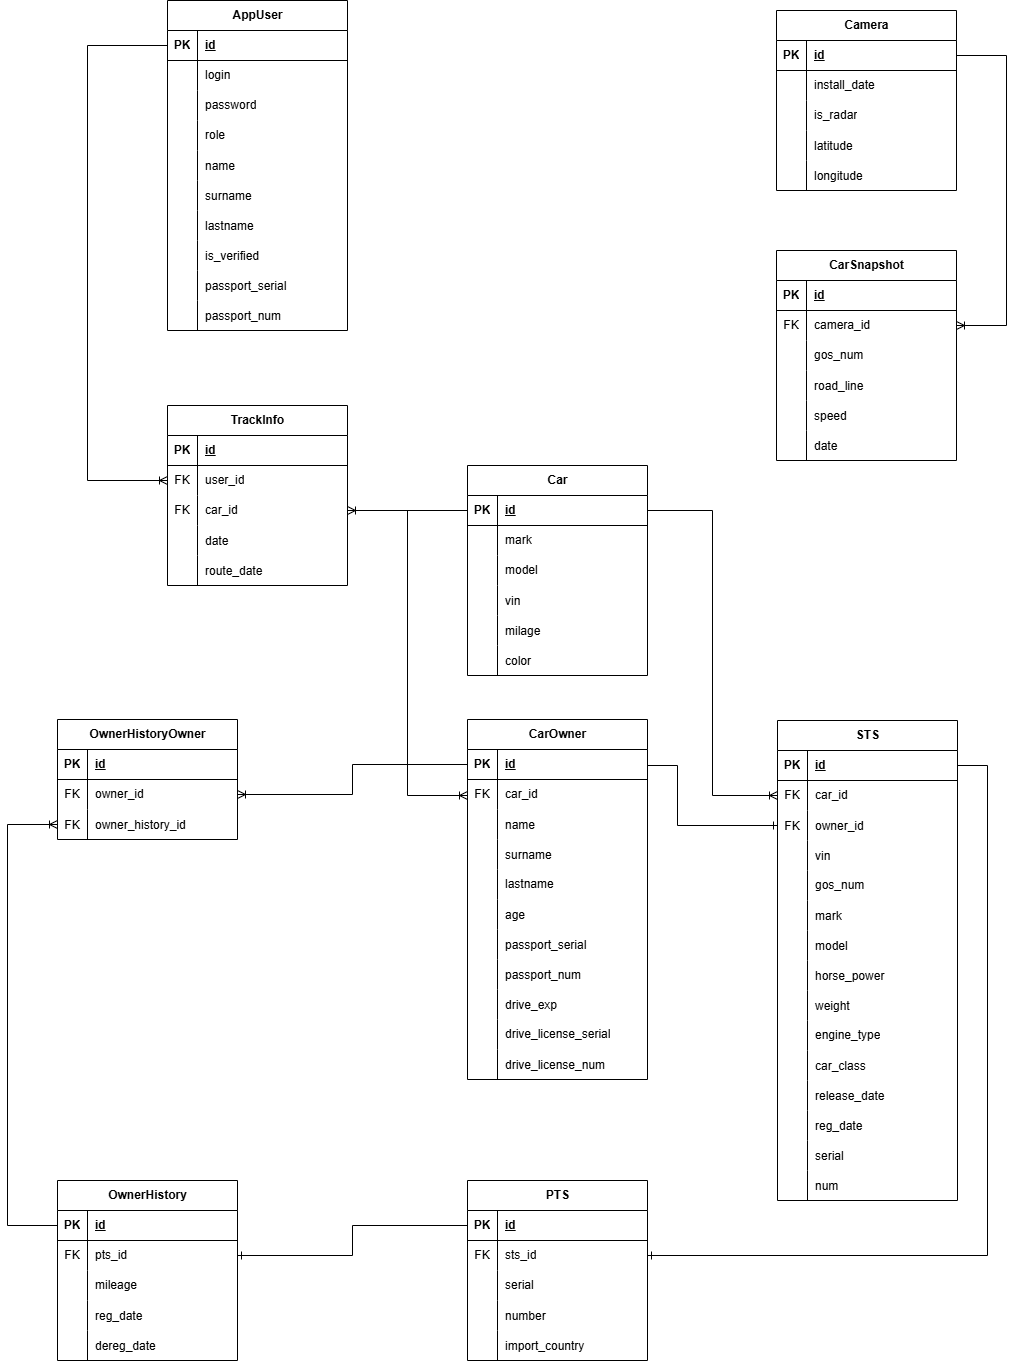
\includegraphics[width=1\linewidth]{images/diograms/tables.png}
    \caption{Диаграмма базы данных}
    \label{fig:tables}
\end{figure}


На таблицах~\ref{table:db:users}~---~\ref{table:db:car_snapshot} приведено описание столбцов таблиц базы данных.

% ПОЛЬЗОВАТЕЛЬ =====================================
\begin{table}[H]
	\begin{center}
		\caption{Информация о столбцах таблицы AppUser}
		\begin{tabular}{|c|c|c|c|}
			\hline
			Столбец & Тип данных & Ограничения & Значение \\
			\hline
			id & Целое число & \makecell{ненулевой, \\ первичный ключ} & \makecell{Идентификатор \\ пользователя} \\
			\hline
			firstname & Строка & ненулевой & Имя \\
			\hline
			surname & Строка & ненулевой & Фамилия \\
			\hline
			lastname & Строка & & Отчество\\
			\hline
			role & Строка & ненулевой & \makecell{Роль \\ пользователя}\\
			\hline
			login & Строка & ненулевой & \makecell{Электронная почта, \\ логин}\\
			\hline
			password & Строка & ненулевой & \makecell{Пароль} \\
			\hline
			is\_verified & Логический тип & ненулевой & \makecell{Верифицирован ли \\ пользователь} \\
			\hline
			passport\_serial & Целое число & ненулевой & Серия паспорта \\
			\hline
            passport\_num & Целое число & ненулевой & Номер паспорта \\
			\hline
		\end{tabular}
		\label{table:db:users}
	\end{center}
\end{table}

% ИНФОРМАЦИЯ ОБ ОТСЛЕЖИВАНИИ =========================

\begin{table}[H]
	\begin{center}
		\caption{Информация о столбцах таблицы TrackInfo}
		\begin{tabular}{|c|c|c|c|}
			\hline
			Столбец & Тип данных & Ограничения & Значение \\
			\hline
			id & Целое число & \makecell{ненулевой, \\ первичный ключ} & \makecell{Идентификатор \\ информации об \\ отслеживании} \\
			\hline
			user\_id & Целое число & \makecell{ненулевой, \\ внешний ключ} & id пользователя \\
			\hline
			car\_id & Целое число & \makecell{ненулевой, \\ внешний ключ} & id автомобиля \\
			\hline
			track\_date & Дата & ненулевой & \makecell{Дата просмотра \\ маршрута}\\
			\hline
			route\_date & Дата & ненулевой & \makecell{Дата \\ просмотренного \\ пути}\\
			\hline
		\end{tabular}
		\label{table:db:track_info}
	\end{center}
\end{table}

% АВТОМОБИЛИ =====================================

\begin{table}[H]
	\begin{center}
		\caption{Информация о столбцах таблицы Car}
		\begin{tabular}{|c|c|c|c|}
			\hline
			Столбец & Тип данных & Ограничения & Значение \\
			\hline
			id & Целое число & \makecell{ненулевой \\ первичный ключ} & \makecell{Идентификатор \\ автомобиля} \\
			\hline
			mark & Строка & ненулевой & Марка \\
			\hline
			model & Строка & ненулевой & Модель \\
			\hline
			vin & Строка & ненулевой & ВИН-номер\\
			\hline
			milage & Строка & \makecell{ненулевой \\ положительное число} & \makecell{Роль \\ пользователя}\\
			\hline
			color & Строка & \makecell{ненулевой} & \makecell{Цвет \\ автомобиля} \\
			\hline
		\end{tabular}
		\label{table:db:cars}
	\end{center}
\end{table}

% птс ================================================

\begin{table}[H]
    \begin{center}
        \caption{Информация о столбцах таблицы PTS}
        \begin{tabular}{|c|c|c|c|}
            \hline
            Столбец & Тип данных & Ограничения & Значение \\
            \hline
            id & Целое число & \makecell{ненулевой, \\ первичный ключ} & \makecell{Идентификатор \\ ПТС} \\
            \hline
            sts\_id & Целое число & \makecell{ненулевой, \\ внешний ключ} & \makecell{Идентификатор \\ СТС} \\
            \hline
            serial & Целое число & ненулевой & Серия ПТС \\
            \hline
            number & Целое число & ненулевой & Номер ПТС \\
            \hline
            import\_country & Строка & ненулевой & \makecell{Страна импорта \\ транспортного \\ средства} \\
            \hline
        \end{tabular}
        \label{table:db:pts}
    \end{center}
\end{table}

% СТС ===============================================

\begin{table}[H]
    \begin{center}
        \caption{Информация о столбцах таблицы STS}
        \begin{tabular}{|c|c|c|c|}
            \hline
            Столбец & Тип данных & Ограничения & Значение \\
            \hline
            id & Целое число & \makecell{ненулевой \\ первичный ключ} & \makecell{Идентификатор \\ СТС} \\
            \hline
            car\_id & Целое число & \makecell{ненулевой, \\ внешний ключ} & \makecell{Идентификатор \\ автомобиля} \\
            \hline
            owner\_id & Целое число & \makecell{ненулевой, \\ внешний ключ} & \makecell{Идентификатор \\ владельца} \\
            \hline
            vin & Строка & ненулевой & \makecell{VIN-номер \\ ТС} \\
            \hline
            gos\_num & Строка & ненулевой & \makecell{Государственный \\ решистрационный \\ знак} \\
            \hline
            mark & Строка & ненулевой & \makecell{Марка ТС} \\
            \hline
            model & Строка & ненулевой & \makecell{Модель ТС} \\
            \hline
            horse\_power & Целое число & \makecell{ненулевой, \\ положительное число} & Мощность (л.с.) \\
            \hline
            weight & Целое число & \makecell{ненулевой, \\ положительное число} & Масса ТС (кг) \\
            \hline
            engine\_type & Строка & ненулевой & \makecell{Тип двигателя} \\
            \hline
            car\_class & Строка & ненулевой & Класс автомобиля \\
            \hline
            release\_date & Дата & ненулевой & Дата выпуска \\
            \hline
            reg\_date & Дата & ненулевой & Дата регистрации \\
            \hline
            serial & Целое число & ненулевой & Серия СТС \\
            \hline
            num & Целое число & ненулевой & Номер СТС \\
            \hline
        \end{tabular}
        \label{table:db:sts}
    \end{center}
\end{table}

% ВЛАДЕЛЬЦЫ =========================================

\begin{table}[H]
    \begin{center}
        \caption{Информация о столбцах таблицы CarOwner}
        \begin{tabular}{|c|c|c|c|}
            \hline
            Столбец & Тип данных & Ограничения & Значение \\
            \hline
            id & Целое число & \makecell{ненулевой \\ первичный ключ} & \makecell{Идентификатор \\ владельца} \\
            \hline
            car\_id & Целое число & \makecell{ненулевой \\ внешний ключ} & \makecell{Идентификатор \\ автомобиля} \\
            \hline
            name & Строка & ненулевой & Имя \\
            \hline
            surname & Строка & ненулевой & Фамилия \\
            \hline
            lastname & Строка &  & Отчество \\
            \hline
            age & Целое число & \makecell{ненулевой, \\ положительное \\ число} & Возраст владельца \\
            \hline
            passport\_serial & Целое число & ненулевой & Серия паспорта \\
            \hline
            passport\_num & Целое число & ненулевой & Номер паспорта \\
            \hline
            drive\_exp & Целое число & \makecell{ненулевой, \\ положительное \\ число} & \makecell{Стаж вождения \\ (в годах)} \\
            \hline
            \makecell{ drive\_ \\ license\_ \\ serial } & Целое число & ненулевой & \makecell{Серия \\ водительского \\ удостоверения} \\
            \hline
            \makecell{drive\_ \\ license\_ \\ num} & Целое число & ненулевой & \makecell{Номер \\ водительского \\ удостоверения} \\
            \hline
        \end{tabular}
        \label{table:db:car_owners}
    \end{center}
\end{table}

% ИСТОРИЯ ВЛАДЕНИЯ ====================================

\begin{table}[H]
    \begin{center}
        \caption{Информация о столбцах таблицы OwnerHistory}
        \begin{tabular}{|c|c|c|c|}
            \hline
            Столбец & Тип данных & Ограничения & Значение \\
            \hline
            id & Целое число & \makecell{ненулевой, \\ первичный ключ} & \makecell{Идентификатор \\ истории \\ владельцев} \\
            \hline
            pts\_id & Целое число & \makecell{ненулевой, \\ внешний ключ} & \makecell{Идентификатор \\ ПТС} \\
            \hline
            mileage & Целое число & \makecell{ненулевой, \\ положительное число} & Пробег (км) \\
            \hline
            reg\_date & Дата & ненулевой & \makecell{Дата \\ регистрации} \\
            \hline
            dereg\_date & Дата & & \makecell{Дата снятия \\ с учета} \\
            \hline
        \end{tabular}
        \label{table:db:owner_history}
    \end{center}
\end{table}

% СВЯЗЬ ИСТОРИИ ВЛАДЕЛЬЦЕВ И ВЛАДЕЛЬЦЕВ ===============

\begin{table}[H]
    \begin{center}
        \caption{Информация о столбцах таблицы OwnerHistoryOwner}
        \begin{tabular}{|c|c|c|c|}
            \hline
            Столбец & Тип данных & Ограничения & Значение \\
            \hline
            id & Целое число & \makecell{ненулевой, \\ первичный ключ} & \makecell{Идентификатор} \\
            \hline
            owner\_id & Целое число & \makecell{ненулевой, \\ внешний ключ} & \makecell{Идентификатор \\ владельца} \\
            \hline
            \makecell{owner\_ \\history\_ \\id} & Целое число & \makecell{ненулевой, \\ внешний ключ} & \makecell{Идентификатор \\ записи истории} \\
            \hline
        \end{tabular}
        \label{table:db:owner_history_owner}
    \end{center}
\end{table}

% КАМЕРА ==============================================

\begin{table}[H]
    \begin{center}
        \caption{Информация о столбцах таблицы Camera (Камеры)}
        \begin{tabular}{|c|c|c|c|}
            \hline
            Столбец & Тип данных & Ограничения & Значение \\
            \hline
            id & Целое число & \makecell{ненулевой, \\ первичный ключ} & \makecell{Идентификатор \\ камеры} \\
            \hline
            install\_date & Дата & ненулевой & Дата установки \\
            \hline
            is\_radar & Логический тип & ненулевой & \makecell{Есть ли \\ радаром} \\
            \hline
            latitude & Вещественное число & ненулевой & Широта \\
            \hline
            longitude & Вещественное число & ненулевой & Долгота \\
            \hline
        \end{tabular}
        \label{table:db:camera}
    \end{center}
\end{table}

% СНИМКИ АВТО =========================================

\begin{table}[H]
    \begin{center}
        \caption{Информация о столбцах таблицы CarSnapshot (Снимки камер)}
        \begin{tabular}{|c|c|c|c|}
            \hline
            Столбец & Тип данных & Ограничения & Значение \\
            \hline
            id & Целое число & \makecell{ненулевой, \\ первичный ключ} & \makecell{Идентификатор \\ снимка} \\
            \hline
            camera\_id & Целое число & \makecell{ненулевой, \\ внешний ключ} & \makecell{Идентификатор \\ камеры} \\
            \hline
            gos\_num & Строка & ненулевой & \makecell{ГРЗ ТС \\ на снимке} \\
            \hline
            road\_line & Целое число & \makecell{ненулевой, \\ положительное число} & Полоса движения \\
            \hline
            speed & Целое число & \makecell{ненулевой, \\ положительное число} & Скорость (км/ч) \\
            \hline
            \makecell{snap\_ \\ datetime} & Дата и время & ненулевой & \makecell{Дата и время \\ снимка} \\
            \hline
        \end{tabular}
        \label{table:db:car_snapshot}
    \end{center}
\end{table}

\section{Описание функции базы данных}

В рамках базы данных будет присутствовать функция верификации пользователя. В качестве входных параметров функции подаются id пользователя, серия и номер паспорта. В случае успеха функция обновит паспортные данные у пользователя с заданным id. На рисунке~\ref{fig:proc} представлена схема функции
верификация пользователя.

\begin{figure}[H]
    \centering
    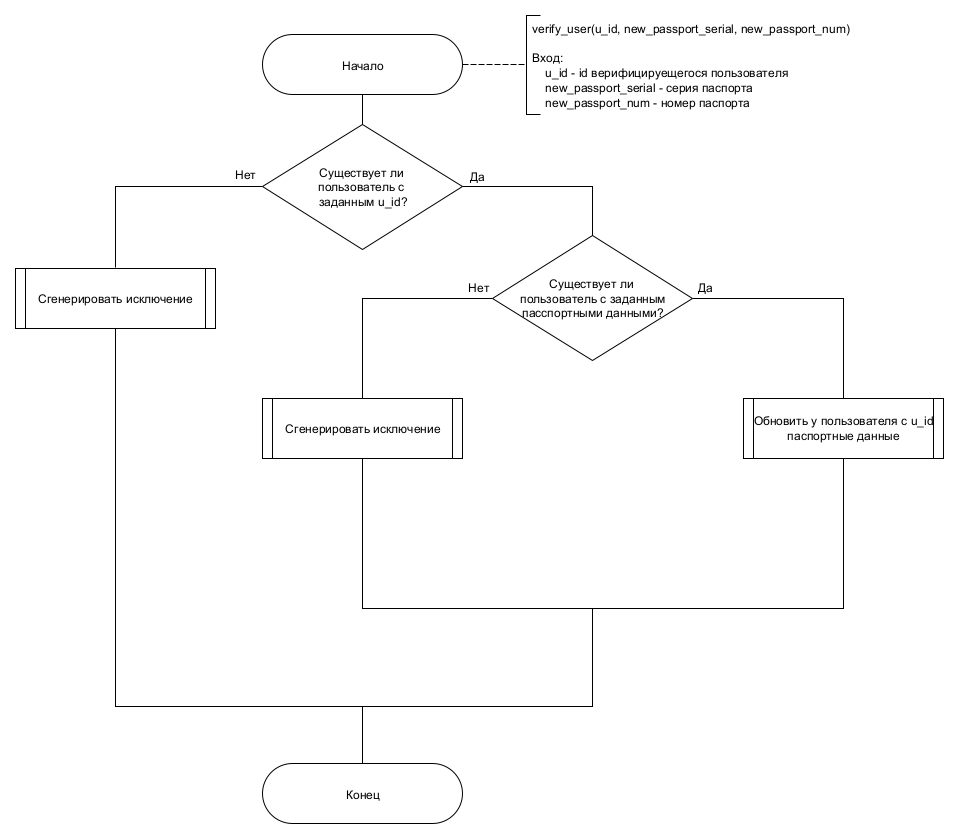
\includegraphics[width=1\linewidth]{images/diograms/procedure_scheme.png}
    \caption{Схема функции верификации пользователя}
    \label{fig:proc}
\end{figure}

\section{Описание ролей базы данных}

Для обеспечения безопасности сервера баз данных необходимо определить следующие пользовательские роли:

\begin{enumerate}
    \item Пользователь имеет права для чтения своих данных из таблиц автомобилей и снимков.
    \item Оператор имеет права для чтения записей из всех таблиц кроме таблицы отслеживания маршрутов автомобилей.
    \item Аудит имеет права для чтения записей из всех таблиц кроме таблиц камер и снимков.
\end{enumerate}

\paragraph*{ВЫВОД} ${}$ \\

В этом разделе представлена диаграмма разрабатываемой базы данных, выполнено описание ее сущностей и ограничений целостности, а также описаны проектируемая процедура и ролевые модели.
